\justifying
\NSFCBodyText

\subsubsection{研究背景与意义}
\textbf{开放课题正文工作稿：本稿借用现有正文版式组织研究内容，正式申报须转入实验室官方申请书。}

矿山开采、堆置与复垦会改变地表覆盖及其空间边界。遥感影像能够提供跨区域的地表观测，但要把两期影像中的差异转化为可供复核的变化范围，还需区分真实地物变化与光照、地表湿度、植被状态等外观差异。全球矿山用地数据已使矿业活动的空间分布获得较系统的刻画\cite{Maus2020Mining,Maus2022Mining}；矿山变化检测进一步把研究对象从单期范围识别推进到两期变化定位\cite{Yu2024MineNetCD}。对矿山地质环境监测而言，清楚标示何处发生可观测变化、哪些判断容易出错，有助于减少逐幅筛查的工作量，也为后续专业解释提供可追溯的影像线索。

本课题以“矿山地表扰动遥感变化检测的跨域泛化与可信评估研究”为工作题，面向中南大学有色金属成矿预测与地质环境监测教育部重点实验室开放课题的矿山地质环境监测方向。研究对象限定为公开影像及变化标签能够支持的地表覆盖和矿山足迹变化。“跨域泛化”主要指模型在未参与训练、选择及校准的矿区上保持判别能力；“可信评估”指概率与错误相符程度、错误区域识别以及固定工作量下的复核效用。二值变化标注不能直接支持污染程度、沉降风险或生态修复成效判定，此类环境解释需要相应观测与专业证据。

矿区之间的地貌、背景地物和观测条件差异，为变化检测带来两类相互关联的问题。其一，背景外观发生差异时，模型可能产生误报；对跨时相特征施加过强的一致性要求，又可能削弱真实细小变化。其二，即使平均检测指标尚可，模型仍可能在部分新矿区给出高置信度错误。若复核只依据预测变化区或最高不确定区域，模型确信“未变化”的漏检会被遗漏。因此，研究需要同时回答约束施于何处、在什么条件下有效，以及错误能否在有限复核面积内被发现。判断这些关系需要分组对照，并检查具体误报与漏检。

上述研究需求及两类差异的关系如图\ref{fig:mct-background}所示。
\begin{figure}[!htbp]
  \centering
  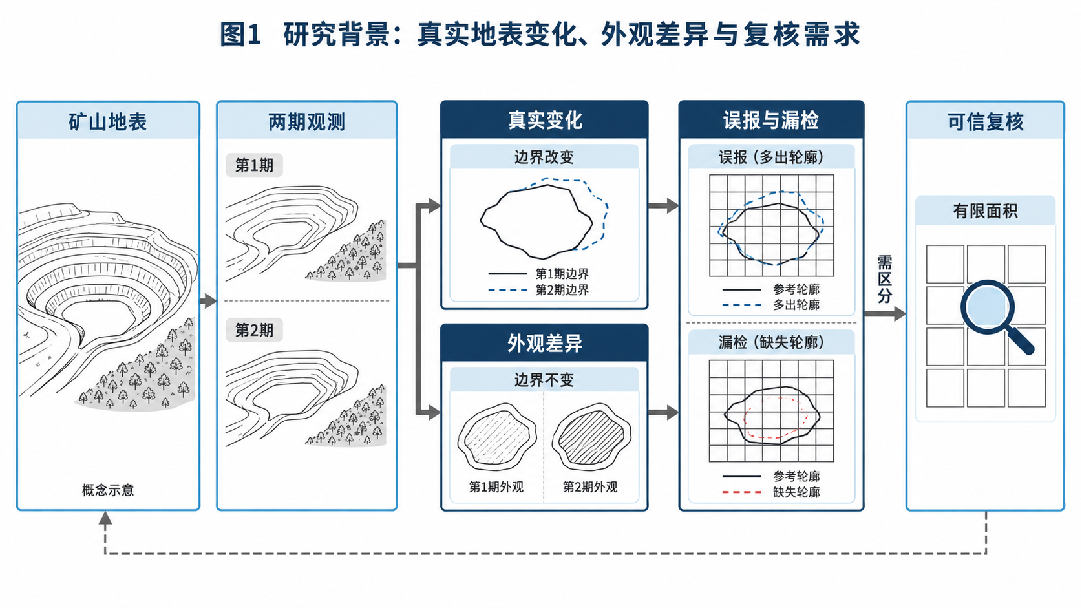
\includegraphics[width=\linewidth,trim=0 0 0 12mm,clip]{figures/F01_research_background.pdf}
  \captionsetup{justification=justified,singlelinecheck=false}
  \caption{研究背景：真实地表变化、外观差异与复核需求。场景、轮廓与复核反馈均为概念示意，用于说明需要区分的观测差异与错误，不表示已验证的误差归因。}
  \label{fig:mct-background}
\end{figure}

\subsubsection{国内外研究现状及发展动态分析}
\textbf{（1）矿山公开数据正在从范围制图走向变化及年度足迹分析。}
MineNetCD覆盖100个全球矿区，包含超过7万对双时相切片及像素级变化标注，并提供ChangeFFT等基准配置。其原论文已按矿区以60\%/10\%/30\%划分训练、验证与测试\cite{Yu2024MineNetCD}，因此矿区隔离本身是本研究应沿用的评测基础。该数据的时相间隔较长，适合研究两期之间的变化范围，不能据此开展逐月事件定位或实时预警。EuroMineNet进一步提供欧盟133个矿区2015—2024年的Sentinel-2年度观测与足迹标签，也采用矿区分组划分\cite{Yu2026EuroMineNet}。两者的分辨率、波段、时相间隔和标签含义存在差别，直接比较其变化交并比（IoU）不能单独解释域偏移。全球铜矿边界与属性数据可辅助核对有色金属矿案例\cite{Li2025Copper}，但单期边界不能充当双时相变化真值。

\textbf{（2）变化检测已形成多类表征方法，背景约束需要面对强近邻比较。}
早期全卷积孪生网络通过双分支特征差异实现变化定位\cite{Daudt2018Siamese}。SNUNet-CD利用密集连接与多尺度交互\cite{Fang2022SNUNet}，BIT与ChangeFormer分别探索语义标记建模及层次Transformer结构\cite{Chen2022BIT,Bandara2022ChangeFormer}，ChangeMamba将状态空间建模用于遥感变化检测\cite{Chen2024ChangeMamba}。这些方法可作为骨干与比较对象。比较时需控制模型容量、上下文范围和训练配置，才能识别矿山任务中的方法增量。

与本项目最接近的工作已涉及一致性和域泛化。FCCDN通过特征约束促进变化判别\cite{Chen2022FCCDN}；DonaNet结合域风格处理、跨时相风格变换及一致性学习，旨在缓解伪变化与跨域泛化问题\cite{Zang2025DonaNet}；CDDGNet进一步研究变化信息与域信息的解耦\cite{Zhao2026CDDG}。因此，泛化变化检测、特征约束或域特征解耦均不能单独作为本项目的创新。本课题拟检验的一项增量是：当一致性约束覆盖真实变化像素时，是否出现可测量的变化敏感性损失；把约束限定于训练标签确认的稳定区，能否在特定干扰条件下缓解这一损失。仅证明增加一个掩码后总体分数上升不足以支持该解释，还需排除约束面积、强度、空间形状及平滑效应的影响。

\textbf{（3）跨域研究要求区分泛化、适应与评测选择。}
通用域泛化研究说明，模型选择与评估协议会影响方法比较，简单基线和一致的选择规则不可省略\cite{Gulrajani2021DomainBed}；MixStyle从特征统计混合研究外观变化的表征学习\cite{Zhou2021MixStyle}，WILDS则通过现实分布变化任务强调域偏移的多样性\cite{Koh2021WILDS}。在遥感变化检测中，AWDA使用目标域无标签数据进行适应\cite{AWDA2025}，其可用信息与不接触目标域数据的纯泛化不同。本项目将这类方法按训练信息分组报告，不将不同信息条件下的结果排成单一优劣次序。

空间数据还存在相邻样本依赖。相关研究讨论了结构化交叉验证、空间预测与插值/外推目标之间的关系\cite{Roberts2017CV,Valavi2019BlockCV,Mila2022Nearest}；遥感制图实例显示，验证方式可能显著影响所报告的预测表现\cite{Ploton2020Spatial}。这些证据支持本课题审计矿区、场景和切片来源，但不能用来指认MineNetCD官方划分已经泄漏。拟分别保留官方协议复现结果与新增校准划分下的结果，所有主比较方法共享相同的训练、选择及测试矿区。

\textbf{（4）校准质量与复核价值需要分别验证。}
温度缩放可作为深度网络概率校准的简单基线\cite{Guo2017Calibration}。分布偏移下的不确定性研究表明，源分布表现不能保证新分布上的可靠性\cite{Ovadia2019Uncertainty}；模型架构与校准的关系也并非“模型越新越不可靠”这一单向规律\cite{Minderer2021Calibration}。遥感变化检测已有利用不确定性描述或改进预测的工作\cite{Li2025Uncertainty}，故输出不确定性图不构成独立创新。温度缩放改变概率尺度，在一些排序定义下未必改变样本顺序；本项目将概率误差下降与错误排序改善作为两项独立结果。

选择性预测通过接受或拒绝部分结果研究风险与覆盖之间的关系\cite{Geifman2019SelectiveNet,Gangrade2021Selective,Franc2023Reject}。这一思路可用于组织人工复核，但像素分类风险与真实复核工作量并不等价：邻近错误可能集中在同一窗口，零散错误则可能需要多次查看；仅报告保留区准确率还可能掩盖未选中区域的漏检。矿山变化复核应在整幅有效区域上分配固定面积预算，同时报告误报、漏检与真实变化覆盖，才能判断排序信息是否具有使用价值。

\subsubsection{现有研究的不足}
\textbf{第一，一致性约束的收益与损伤还需在矿山任务中分开识别。}
已有工作给出通用约束方法，尚不能由其总体指标确定本课题数据中哪些误差主要来自背景外观、哪些来自真实变化的特征收缩。若只报告整体IoU，背景像素数量优势可能掩盖细小变化受损。需要把约束区域和约束强度分开控制，并以变化尺度和外观差异的预定义分层检验适用条件；这些分层反映观测关联，其机制解释还需受控扰动和约束污染实验共同支持。

\textbf{第二，可靠性改善能否转化为复核收益仍需直接证据。}
概率校准误差、错误排序和人工复核分别回答不同问题。现有概念与方法不能自动保证新矿区高置信度漏检被发现。需要用包含预测未变化区的统一窗口集合，比较随机、原始熵、校准熵及推理分歧在同等面积下留下的错误，明确理想纠错模拟与真实人员复核的差别。

\textbf{第三，矿山场景中的方法结论需要具有可追溯的外部有效性边界。}
矿区隔离、标签口径和输入适配是建立可信结论的基础。泛化优势若只来自少数大矿区、特定变化尺度或某种标注方式，其适用范围应如实报告。研究重点是找到可复现的条件与反例，而不是在未经对齐的数据集间拼接更大的实验规模。

\subsubsection{关键科学问题与研究切入点}
本项目的中心问题是：\textbf{矿山双时相影像中，一致性约束作用的区域如何影响真实变化与背景差异的可分性，其预测错误能否在未见矿区被有效识别？}围绕这一问题，先判断跨矿区错误的主要来源，再检验稳定区约束的条件性作用，最后评价错误排序的复核价值。三个环节分别提供失效证据、机制证据和使用证据。

核心假说为：在训练监督及计算预算一致的条件下，稳定背景限定的一致性约束可在未见矿区减少误报，并保持细小变化召回。总体收益按矿区主要判据检验；外观差异、变化尺度及约束中变化像素比例如何影响该作用，作为预先规定的条件探索。若等面积随机掩码、同等平滑即可解释收益，或召回损失超过预先约定的非劣界，则该假说得不到支持。稳定背景在此仅指标签确认未变化的有效区域，不预设它具有地质学上的稳定性。

辅助假说为：在独立矿区校准和开发集选择之后，固定多视图推理分歧与概率熵的简洁组合，能够在固定复核面积内比单独指标发现更多错误，并降低未复核区域漏检。其有效性用全图剩余误报和漏检分别检验；优势若仅出现在高复核比例或单个矿区，不扩大为普遍可靠性结论。

当前已完成公开来源与方法近邻核查，并在MineNetCD裁切子样本上完成三组、三个种子的预实验，详见研究基础。背景约束相对全区域约束的降误报伴随总体召回下降，IoU差区间跨零，小变化端点不可估计，尚不支持上述联合假说。项目将以首阶段数据与误差诊断决定是否继续机制实验；若主要瓶颈是配准或标签口径，则优先澄清数据问题，再收敛可回答的问题。预期贡献是给出一致性约束的适用条件及可证伪解释，并形成矿区级、固定复核面积下的检测可靠性证据。
